\documentclass[12pt%
%,draft%
,aspectratio=169%
]{beamer}
%
\usepackage{fontspec}
\defaultfontfeatures{Ligatures=TeX}
%\setsansfont{Liberation Sans}
\usepackage{polyglossia}
\setdefaultlanguage{ngerman}
% Alternative template for talks of the Freie Universität Berlin.
% Created by Leonard R. König, <leonard.koenig@fu-berlin.de> following the
% guidelines on www.fu-berlin.de/cd
%
% (c) Leonard König, CC BY 4.0
%
% This template was written against UTF-8 capable LaTeX engines, specifically
% LuaLaTeX.

% Trying to get rather close to the ppt/odp template:
%  http://www.fu-berlin.de/sites/cd/downloads_container/PowerPoint_Praesentation_Anleitung.pdf

%%% font styles
\setbeamerfont{frametitle}{series=\bfseries}
\setbeamerfont{footline}{series=\bfseries}
\setbeamerfont{headline}{series=\bfseries}
\setbeamerfont{alerted text}{series=\bfseries}
%%%

% colordefs
\definecolor{fu_darkblue}{RGB}{0,51,102}
\definecolor{fu_seablue}{RGB}{0,102,204}
\definecolor{fu_lightblue}{RGB}{204,214,224}
\definecolor{fu_green}{RGB}{153,204,0}
\definecolor{fu_lightgrey}{RGB}{128,128,128}
\definecolor{fu_grey}{RGB}{95,95,95}
%
\definecolor{fu_red}{RGB}{204, 0, 0} % red text (used by \alert)
%%% end colordefs

%%% colors
\setbeamercolor*{title}{fg=fu_darkblue}
\setbeamercolor*{subtitle}{fg=fu_seablue}
\setbeamercolor*{frametitle}{fg=fu_darkblue}
\setbeamercolor*{footline}{fg=fu_grey,bg=fu_lightblue}
\setbeamercolor*{headline}{fg=fu_grey}

\setbeamercolor*{normal text}{fg=black}
\setbeamercolor*{alerted text}{fg=fu_red}
\setbeamercolor*{example text}{fg=fu_green}
\setbeamercolor*{structure}{fg=fu_darkblue}

\setbeamercolor*{block title}{fg=white,bg=black!50}
\setbeamercolor*{block title alerted}{fg=white,bg=black!50}
\setbeamercolor*{block title example}{fg=white,bg=black!50}

\setbeamercolor*{block body}{bg=black!10}
\setbeamercolor*{block body alerted}{bg=black!10}
\setbeamercolor*{block body example}{bg=black!10}

\setbeamercolor{bibliography entry author}{fg=fu_darkblue}

\setbeamercolor{item}{fg=fu_darkblue}
\setbeamercolor{navigation symbols}{fg=fu_lightgrey,bg=fu_grey}
%%% end colors

%%% title page
% Display logo (if exists) and right next to it, put our title + subtitle
\defbeamertemplate*{title page}{fu_titlepage}
{%
	\hskip .3\textheight
	\begin{minipage}[.4\textheight]{\textwidth}
		\begin{minipage}[.4\textheight]{0.25\textwidth}
			\inserttitlegraphic
		\end{minipage}%
		\begin{minipage}[.4\textheight]{0.75\textwidth}
			\begin{beamercolorbox}{title}
				\usebeamerfont{title}\inserttitle\par%
			\end{beamercolorbox}
			\vfill
			\ifx\insertsubtitle
				\@empty%
			\else
				\begin{beamercolorbox}{subtitle}
					\usebeamerfont{subtitle}\insertsubtitle\par
				\end{beamercolorbox}
			\fi
		\end{minipage}
	\end{minipage}%
	\hskip .3\textheight
}
%%% end title page

%%% headline
% display title, author and institute on the left;
% logo on the right.
\newcommand{\headlinetext}
{%
	\inserttitle\\[0.3em]%
	\insertauthor, %
	\insertshortinstitute
}
\newlength{\headlinewidth}
\setlength{\headlinewidth}{\paperwidth}
\addtolength{\headlinewidth}{-2\marginparsep}
\setbeamertemplate{headline}
{%
	\begin{beamercolorbox}[wd=\paperwidth]{headline}%
		\vskip5pt
		{\hspace*{\marginparsep}}%
		\parbox{.5\headlinewidth}
		{%
			\usebeamertemplate{title in head/foot}%
			\headlinetext%
		}%
		\begin{minipage}{.5\headlinewidth}%
			\hfill\usebeamertemplate*{logo}
		\end{minipage}%
		{\hspace*{\marginparsep}}%
	\end{beamercolorbox}%
}
%%% end headline

%%% footline
% title + date on the left, frame number on the right
\newcommand{\footlinetext}
{%
	\usebeamerfont{shorttitle}\insertshorttitle, %
	\usebeamerfont{shortdate}\insertshortdate
}
\setbeamertemplate{footline}
{%
	\begin{beamercolorbox}{footline}
		\vskip2pt
		\hspace{\marginparsep}%
		\footlinetext\hfill%
		\insertframenumber%
		\hspace{\marginparsep}
		\vskip2pt
	\end{beamercolorbox}%
}
%%% end footline

% don't use default templates for sidebars
\setbeamertemplate{sidebar right}{}
\setbeamertemplate{sidebar left}{}
\setbeamertemplate{title page}[fu_titlepage]
\usepackage{amsmath}
\usepackage{amsfonts}
\usepackage{amssymb}
\usepackage{graphicx}
\usepackage{algorithm}
\usepackage[noend]{algpseudocode}
%\usepackage{algorithmic}
\usepackage{tikz}
\usetikzlibrary{arrows,shapes,automata,petri,positioning,calc}
\usepackage{graphicx}
\usepackage{subfig}
\usepackage{pgfplots}
\usepackage{venndiagram}
\usepackage{ stmaryrd }


\usepackage{luacode} % for '\luaexec' macro
%% Define a LaTeX "wrapper" macro:
\newcommand\bitwiseXOR[2]{\luaexec{tex.sprint((#1)~(#2))}}
\newcommand\bitwiseAND[2]{\luaexec{tex.sprint((#1)&(#2))}}
\newcommand\bitwiseOR[2]{\luaexec{tex.sprint((#1)|(#2))}}


\pgfplotsset{
    standard/.style={%Axis format configuration
        axis x line=middle,
        axis y line=middle,
        enlarge x limits=0.15,
        enlarge y limits=0.15,
        every axis x label/.style={at={(current axis.right of origin)},anchor=north west},
        every axis y label/.style={at={(current axis.above origin)},anchor=north east},
        every axis plot post/.style={mark options={fill=white}}
        }
    }


\author{Benjamin Tröster}
\title[Schalttechnik \& Logikgatter]{Schalttechnik \& Logikgatter}
%\subtitle[Markov Models]{...}
%\pgfdeclareimage{titlegraphic}{../res/dwarf_logo2.png}
%\titlegraphic{\pgfuseimage{titlegraphic}}
%\date{}
%\subject{}
%
% FU settings
\institute[HTW Berlin]{Hochschule für Technik und Wirtschaft Berlin}
%\pgfdeclareimage[height=0.9cm]{logo}{../res/dwarf_logo}
%\logo{\pgfuseimage{logo}}
%
\usepackage[
backend=biber,
citestyle=alphabetic,bibstyle=authoryear
]{biblatex}
\addbibresource{sources.bib}


\begin{document}

\begin{frame}
\titlepage
\end{frame}

\begin{frame}{Fahrplan}
\tableofcontents[hideothersubsections]
\end{frame}

\section{Recap}
\begin{frame}{Bool'sche Algebra nach Huntington (\textbf{Wichtig!})}
\begin{definition}
Die bool'sche Algebra nach Huntington ist definiert als Menge $\mathcal{V}: \{0,1\}$ mit den Verknüpfungen $\cdot (\land), + (\lor)$, sodass $\mathcal{V} \times \mathcal{V} \to \mathcal{V}$, also $\{0,1\} \times \{0,1\} \to \{0,1\}$. 
\end{definition}
\begin{itemize}
	\item Kommutativgesetze (K): $a \cdot b = b \cdot a$ bzw. $a + b = b + a$
	\item Distributivgesetze (D): $a \cdot (b + c) = (a \cdot b) + (a \cdot c)$ bzw. $a + (b \cdot c) = (a + b) \cdot (a + c)$
	\item Neutrale Elemente (N): $ \exists e, n \in \mathcal{V}$ mit  $a \cdot e = a$ und $a + n = a$
	\item Inverse Elemente (I): $\forall a \in \mathcal{V}$ existiert ein $a'$ mit $a \cdot a'= n$ und $a + a' = e$
\end{itemize}
Übernommen von \cite{barnett2013boolean} bzw. \cite{hoffmann2020grundlagen}
\end{frame}

\begin{frame}{Notation und Operatorenbindung}
\begin{itemize}
	\item Syntactic Sugar (Ableitungen aus Basisverknüpfungen)
	\begin{itemize}
		\item $(a \Rightarrow b)$ für $(\neg a \lor b)$ -- Implikation
		\item $(a \Leftarrow b)$ für $(b \Rightarrow a)$ -- Inversion der Implikation
		\item $(a \Leftrightarrow b)$ für $(a \Rightarrow b) \land (a \Leftarrow b)$ -- Äquivalenz
		\item $(a \oplus b)$ für $\neg (a \Leftrightarrow b)$ -- Antivalenz oder Exklusiv-ODER/XOR
		\item $\neg(a \lor b)$ -- NOR
		\item $\neg (a \land b)$ -- NAND
	\end{itemize}
	\item Bindung der Operatoren 
	\begin{itemize}
		\item $\land$ bindet stärker als $\lor$
		\item $\neg$ bindet stärker als $\land$
	\end{itemize}
	\item Klammerung
	\begin{itemize}
		\item Gleiche Verknüpfungen: linksassoziativ zusammengefasst
	\end{itemize}
\end{itemize}	 
\end{frame}

\begin{frame}{Erfüllbarkeit}
	\begin{definition}[Erfüllbarkeit]
		Sei $\varphi$ ein beliebiger boolescher Ausdruck. $\varphi$ heißt
		\begin{itemize}
			\item erfüllbar, wenn es Werte $x_1, \ldots, x_n$ gibt, mit $\varphi (x_1, \ldots, x_n ) = 1$.
			\item widerlegbar, wenn es Werte $x_1, \ldots, x_n$ gibt, mit $\varphi (x_1, \ldots, x_n) = 0$.
			\item unerfüllbar, wenn $\varphi (x_1 ,\ldots , x_n )$ immer gleich $0$ ist.
			\item allgemeingültig, wenn wenn $\varphi (x_1 ,\ldots , x_n )$ immer gleich $1$ ist.
		\end{itemize}
		Einen allgemeingültigen Ausdruck bezeichnen wir auch als \textbf{Tautologie}.
	\end{definition}
\end{frame}


\begin{frame}{Negationstheorem}
\begin{theorem}[Negationstheorem]
Sei $f(0, 1, x_1 , \ldots , x_n , \land, \lor, \neg)$ ein boolescher Ausdruck, in dem neben den Konstanten $1$ und $0$ und den Variablen $x_1 ,\ldots, x_n$ die booleschen Operatoren $\land, \lor$ und $\neg$ vorkommen. Dann gilt:
$$
	\overline{f(0, 1, x_1 , \ldots , x_n , \land, \lor, \neg)} = f(1, 0, \overline{x_1}, \ldots ,\overline{x_n} ,\lor, \land, \neg)
$$
\end{theorem}
\end{frame}

\begin{frame}{Dualitätsprinzip}
\begin{theorem}
Sei
$$
\varphi(0, 1, x_1 , \ldots, x_n , \land, \lor, \neg) = \psi(0, 1, x_1 , \ldots, x_n , \land, \lor, \neg)
$$
ein Gesetz der booleschen Algebra, in der neben Variablen und den Konstanten $0$ und $1$ ausschließlich die Elementarverknüpfungen $\neg, \land$ und $\lor$ vorkommen. Dann ist auch die duale Gleichung
$$
\varphi(0, 1, x_1 , \ldots, x_n , \land, \lor, \neg) = \psi(0, 1, x_1 , \ldots, x_n , \land, \lor, \neg)
$$
ein Gesetz der booleschen Algebra.
\end{theorem}
\end{frame}

\begin{frame}{Vollständige Operatorensysteme}
\begin{definition}[Vollständige Operatorensystem]
$\mathcal{M}$ sei eine beliebige Menge von Operatoren. $\mathcal{M}$ ist ein vollständiges Operatorensystem, wenn sich jede boolesche Funktion durch einen Ausdruck beschreiben lässt, in dem neben den Variablen $x_1 , \ldots , x_n$ ausschließlich Operatoren aus $\mathcal{M}$ vorkommen.
\end{definition}
\begin{itemize}
	\item Die Elementaroperatoren $\land, \lor$ und $\neg$ bilden zusammen ein vollständiges Operatorensystem
	\item Die Operatoren NAND und NOR bilden jeder für sich bereits ein vollständiges Operatorensystem
	\item Die Implikation und die $0$ bilden zusammen ebenfalls ein vollständiges Operatorensystem
\end{itemize}
\end{frame}

\begin{frame}{Normalformdarstellungen}
\begin{itemize}
	\item Normalform beschreibt eine eindeutige Darstellung
	\item Vollform: Ausdruck, in dem jede Variable genau einmal vorkommt 
	\item Literal: Teilausdruck, der entweder negierte oder unnegierte Variable darstellt
	\item Wahrheitstafeldarstellung ist eine Art der Normalformdarstellungen
	\item Bool'sche Ausdrücke hingegen sind keine Normalformdarstellung
	\begin{itemize}
		\item Jede bool'sche Funktion durch unendlich viele Ausdrücke beschrieben werden
	\end{itemize}
\end{itemize}
\end{frame}

\begin{frame}{Disjunktive Normalform}
\begin{itemize}
	\item Die disjunktive Normalform (DNF) ist jene Darstellungsart, bei der eine Reihe von Vollkonjunktionen disjunktiv verknüpft wird. Negationen  treten nur in atomarer Form auf.
	\begin{itemize}
		\item $(A \land \neg B \land C) \lor (A \land B \land C) \lor (\neg A \land \neg B \land C)$ 
	\end{itemize}
	\item \item Die konjunktive Normalform (KNF) ist jene Darstellungsart, bei der eine Reihe von Volldisjunktionen konjunktiv verknüpft wird. Negationen treten nur in atomarer Form auf.
	\begin{itemize}
		\item $(\neg A \lor \neg B \lor \neg C) \land (A \lor B \lor C) \land (A \lor \neg B \lor \neg C)$ 
	\end{itemize}
	\item Andere Bezeichnungen:
	\begin{itemize}
		\item Kanonische disjunktive/konjunktive Normalform (KDNF/KKNF)
		\item Vollständige disjunktive/konjunktive Normalform
	\end{itemize}
\end{itemize}
\end{frame}

\begin{frame}{Bitweise logische Operationen}
\begin{center}
$A,B$ seien Bitvektoren, $\circ$ eine beliebige Verknüpfung
\begin{figure}
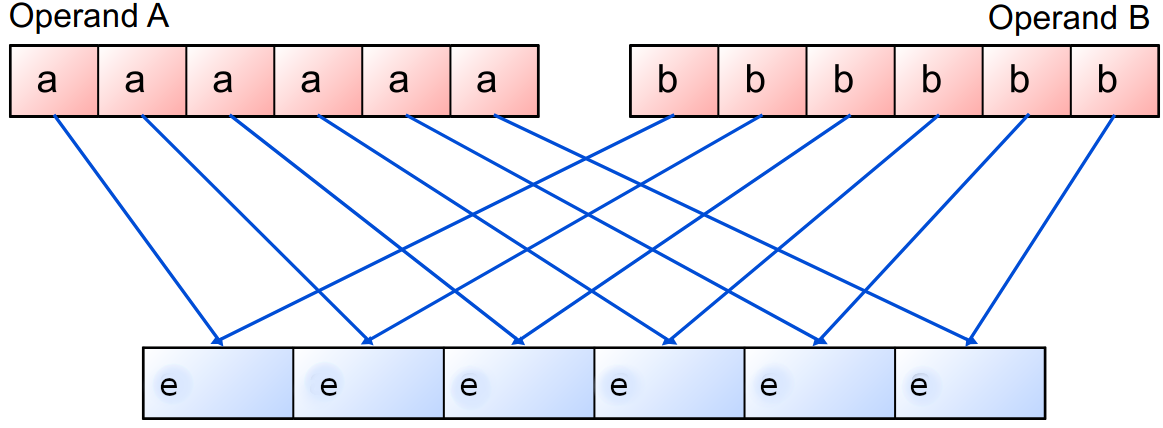
\includegraphics[scale=0.3]{pictures/bitvec}
\end{figure}
Dann erhalten wir als Ergebnis: $E = A \circ B$
\end{center}
\end{frame}

\section{Einleitung}
\begin{frame}{Heute:}
\begin{itemize}
	\item
\end{itemize}

\end{frame}


\section*{Quellen}
\appendix
\begin{frame}[allowframebreaks]
  \frametitle<presentation>{Quellen}
\printbibliography
\end{frame}
\end{document}